\section{わかるらんど}
本章では,我々の開発した『わかるらんど』の機能と使用方法について述べる.

\subsection{ユーザインタフェース}

『わかるらんど』のユーザインタフェースは「ダッシュボード」と「投稿画面」の2つからなり,
画面右上のボタンで切り替えることができる.
図\ref{dashboard}はダッシュボードのスクリーンショットである.
ユーザが投稿したテキストやスタンプや,
各種のセンサのデータなどがリアルタイムに1つの画面に表示されている.
センサのデータなどは自動的に更新され,ユーザのリアクションは図\ref{console}の投稿画面で
ユーザ名を入力し,スタンプを一覧から選んで投稿することで
自分のアイコンの上にオーバーレイ表示される.
ユーザの投稿には表示時間が設定されており,
指定時間が経過すると自動的に投稿が取り下げられるため
いつまでも古い投稿が表示され続けてしまうということはない.
表示時間はユーザがスタンプをクリックする時間の長さで設定される.

% 投稿するスタンプは投稿画面でユーザが自由に追加/削除することができる.

\begin{figure}[h]
\centering
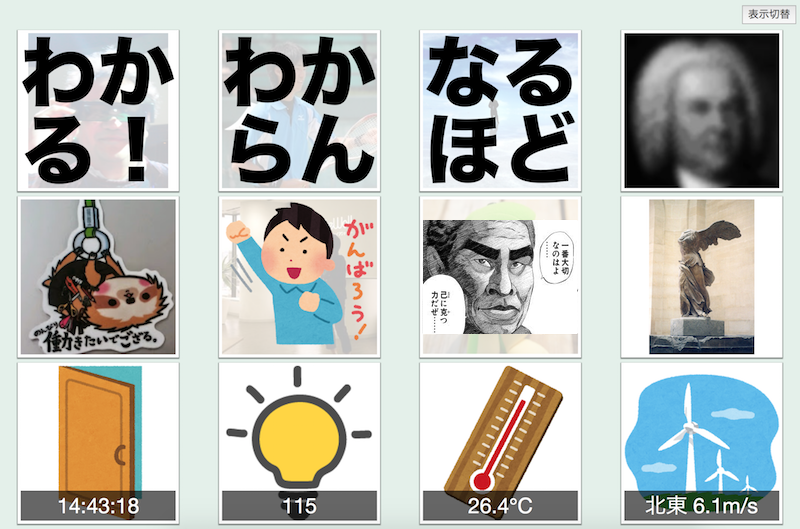
\includegraphics[width=7cm]{images/dashboard.png}
\caption{『わかるらんど』のダッシュボード}
\label{dashboard}
\end{figure}

\begin{figure}[h]
\centering
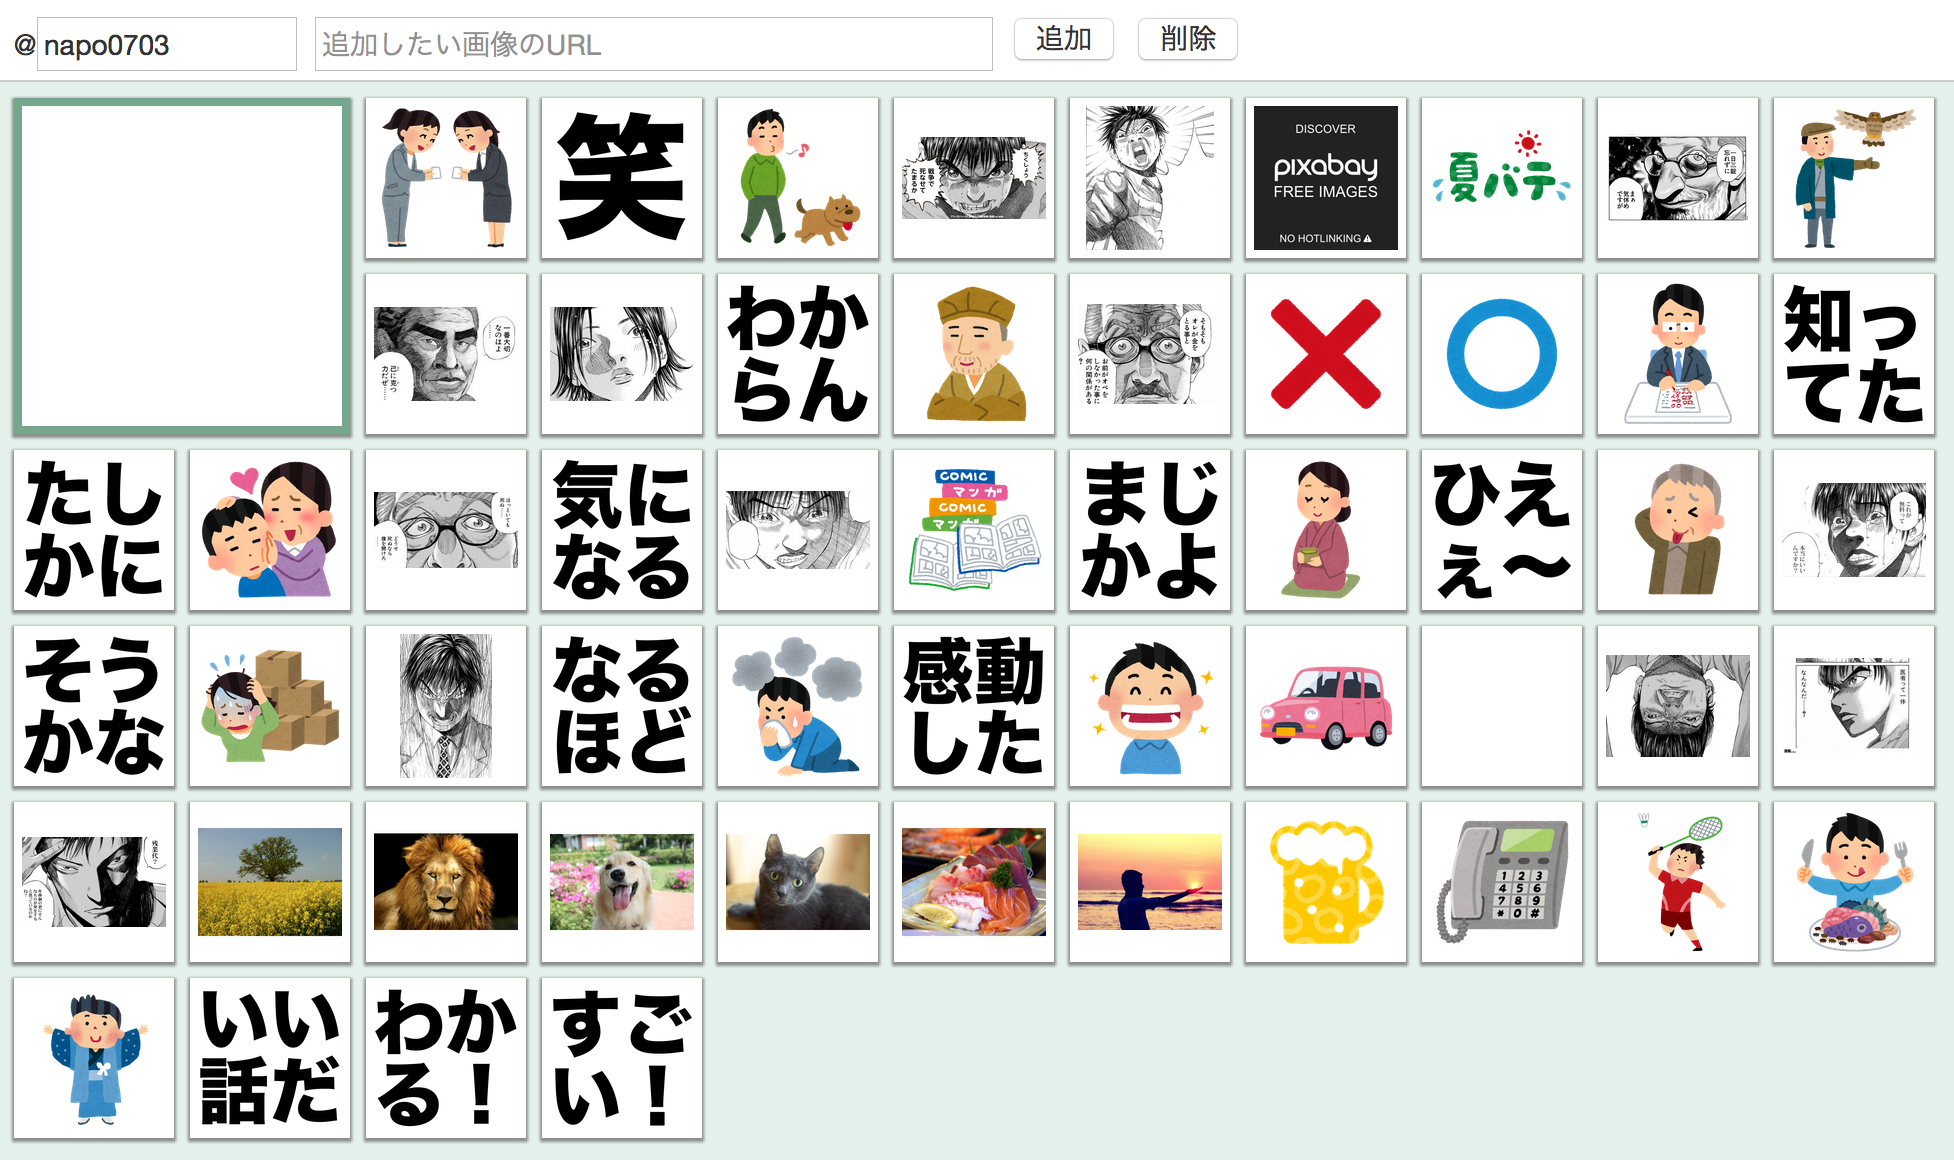
\includegraphics[width=7cm]{images/console.png}
\caption{『わかるらんど』の投稿画面}
\label{console}
\end{figure}

\subsection{表示するユーザとデータの指定}

『わかるらんど』のダッシュボードに表示されるセルは,ユーザのテキストや画像のスタンプを表示する
「リアクション」セルと,センサやWebの情報を表示する「データ」セルの2種類がある(図\ref{cell}).

\begin{figure}[h]
\centering
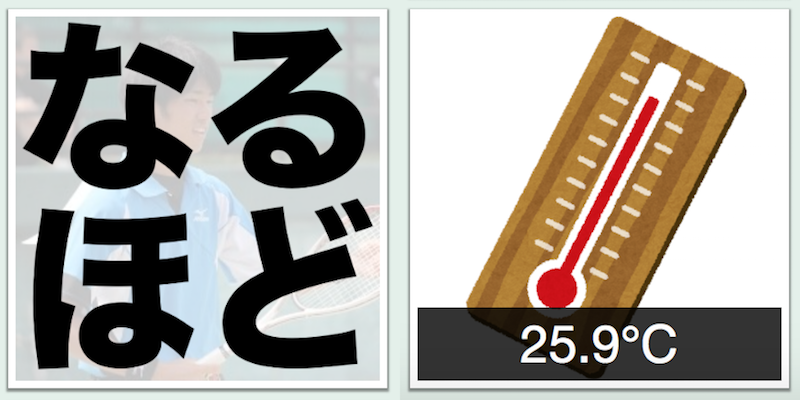
\includegraphics[width=7cm]{images/cell.png}
\caption{リアクション(左)とデータ(右)}
\label{cell}
\end{figure}

ダッシュボードに表示するユーザのリアクションの指定は,
\url{https://wakaruland.com/@napo0703,@masui,@shokai,@dorayaki0}
のようにURLの末尾にカンマ区切りでTwitterのユーザ名を「\url{@}」を付けて書くことで行う.
この場合は図\ref{n_m_s_d}のように\url{@napo0703,@masui,@shokai,@dorayaki0}の4人のユーザのセルが
ダッシュボードに表示される.

\begin{figure}[h]
\centering
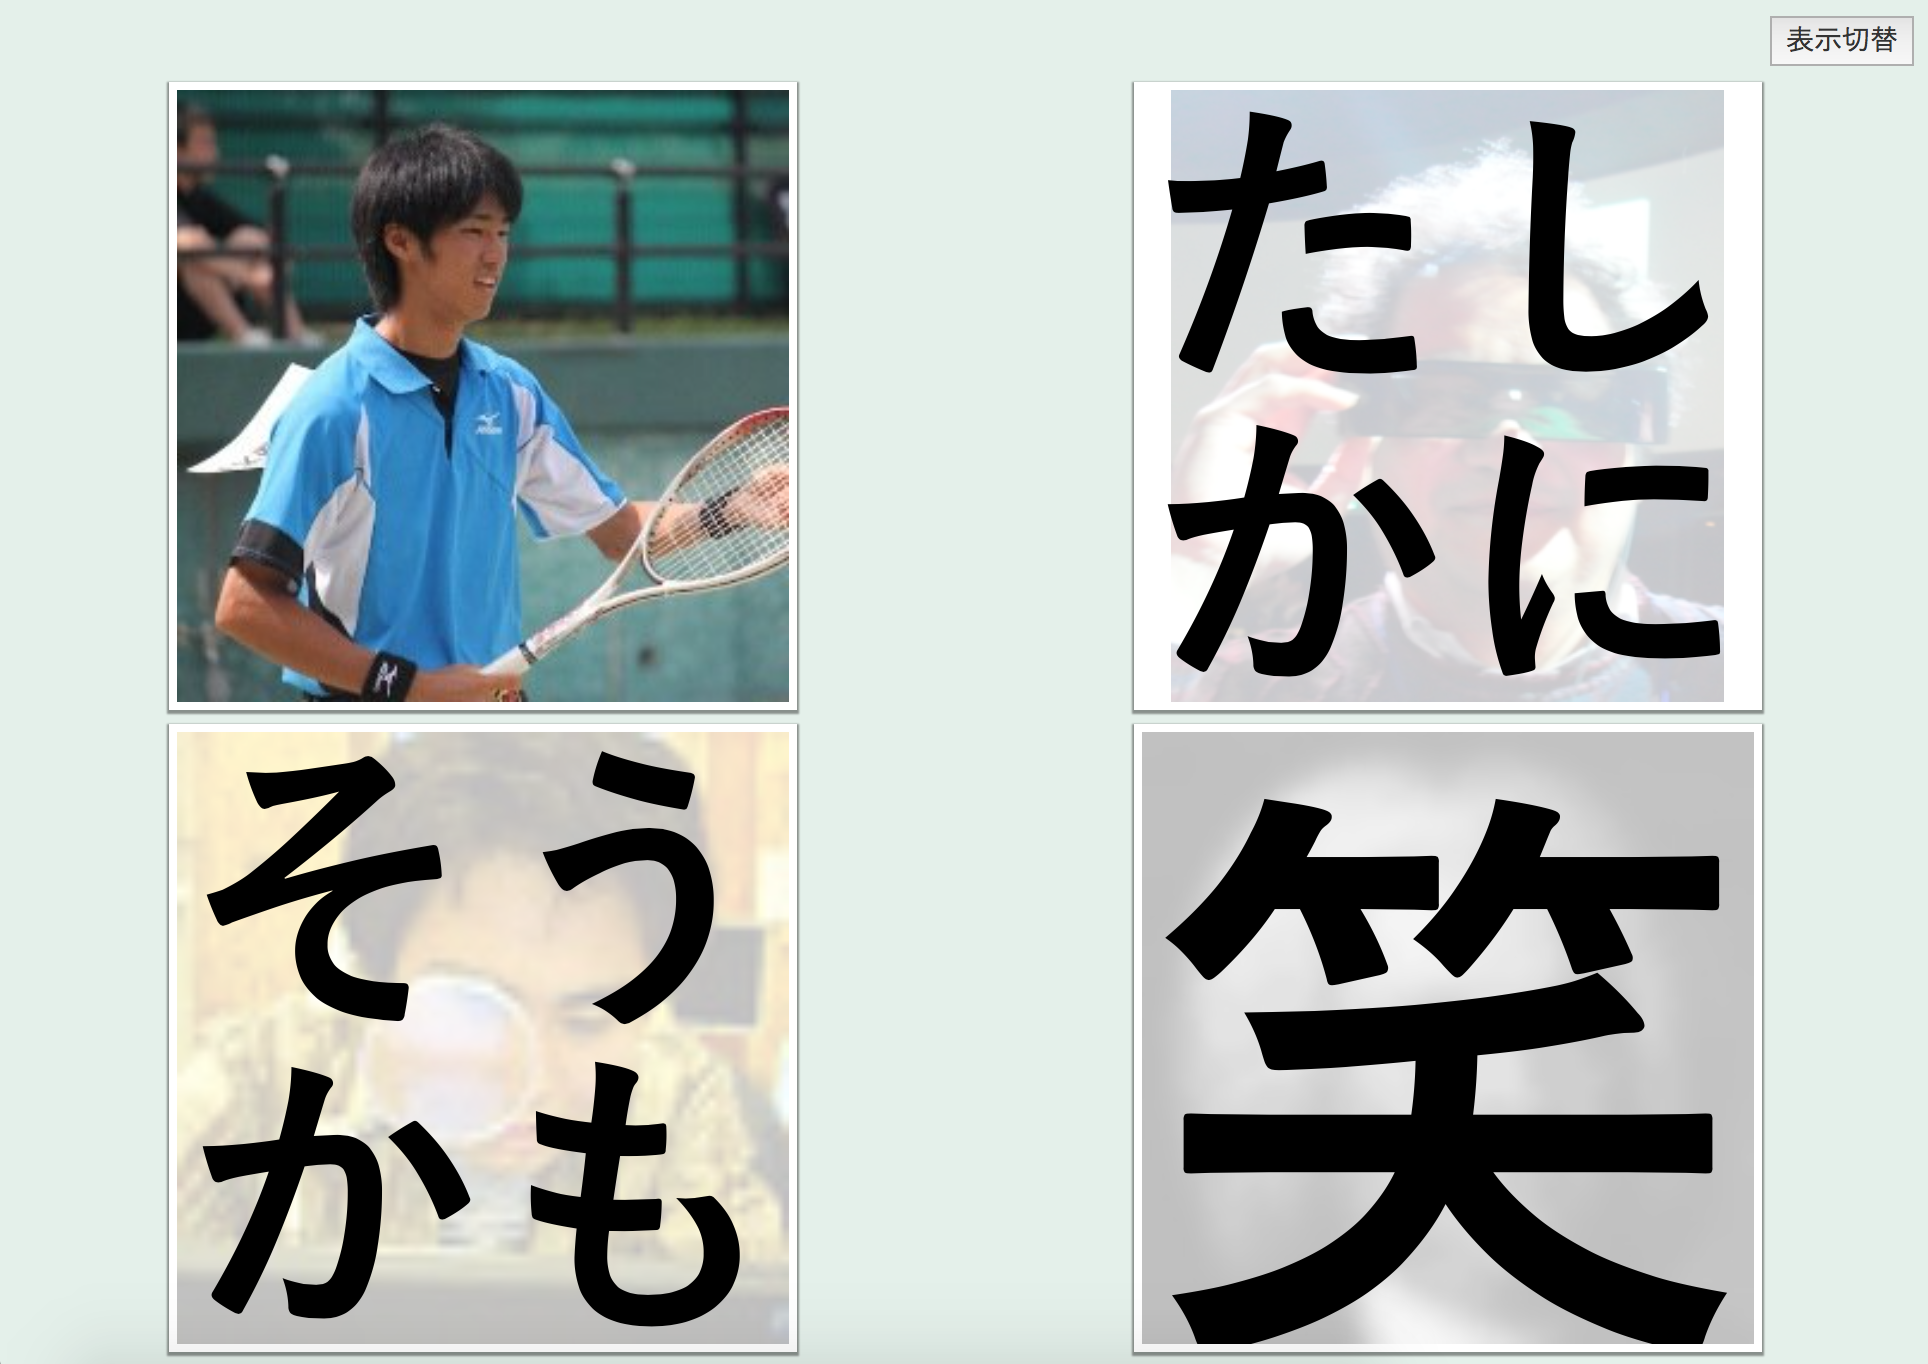
\includegraphics[width=7cm]{images/n_m_s_d.png}
\caption{4人のユーザを表示}
\label{n_m_s_d}
\end{figure}

\url{https://wakaruland.com/weather,temperature,wind}のように「\url{@}」を付けなかった場合は図\ref{w_t_w}のように\url{weather,temperature,wind}の3つがデータのセルとして表示される.

\begin{figure}[h]
\centering
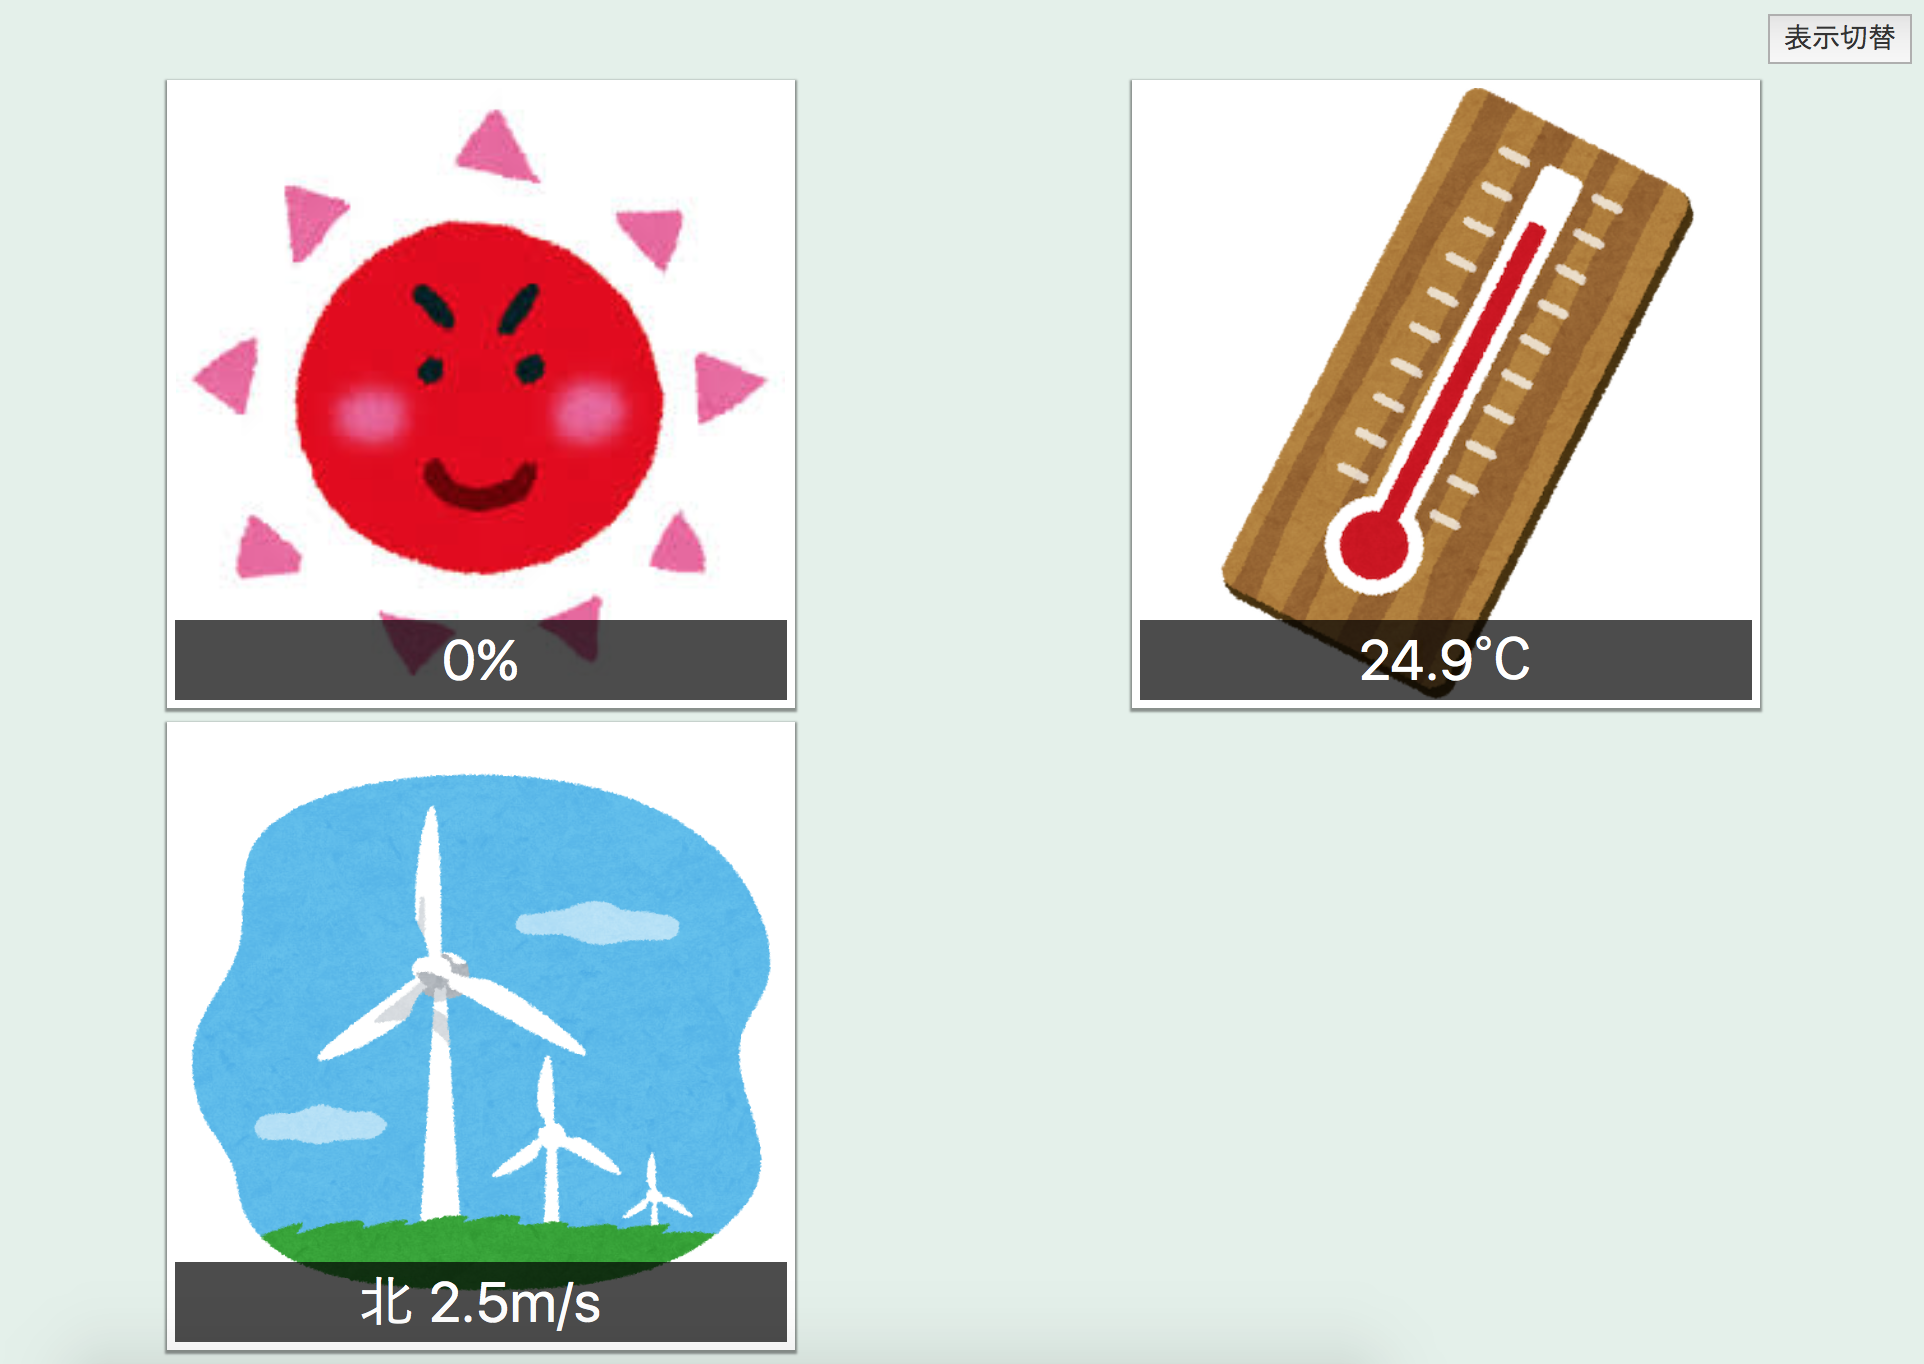
\includegraphics[width=7cm]{images/w_t_w.png}
\caption{3つのデータを表示}
\label{w_t_w}
\end{figure}

また,\url{https://wakaruland.com/@napo0703,weather,@masui,wind,@shokai}のようにリアクションとデータを合わせて表示させることも可能である(図\ref{n_w_m_w_s}).

\begin{figure}[h]
\centering
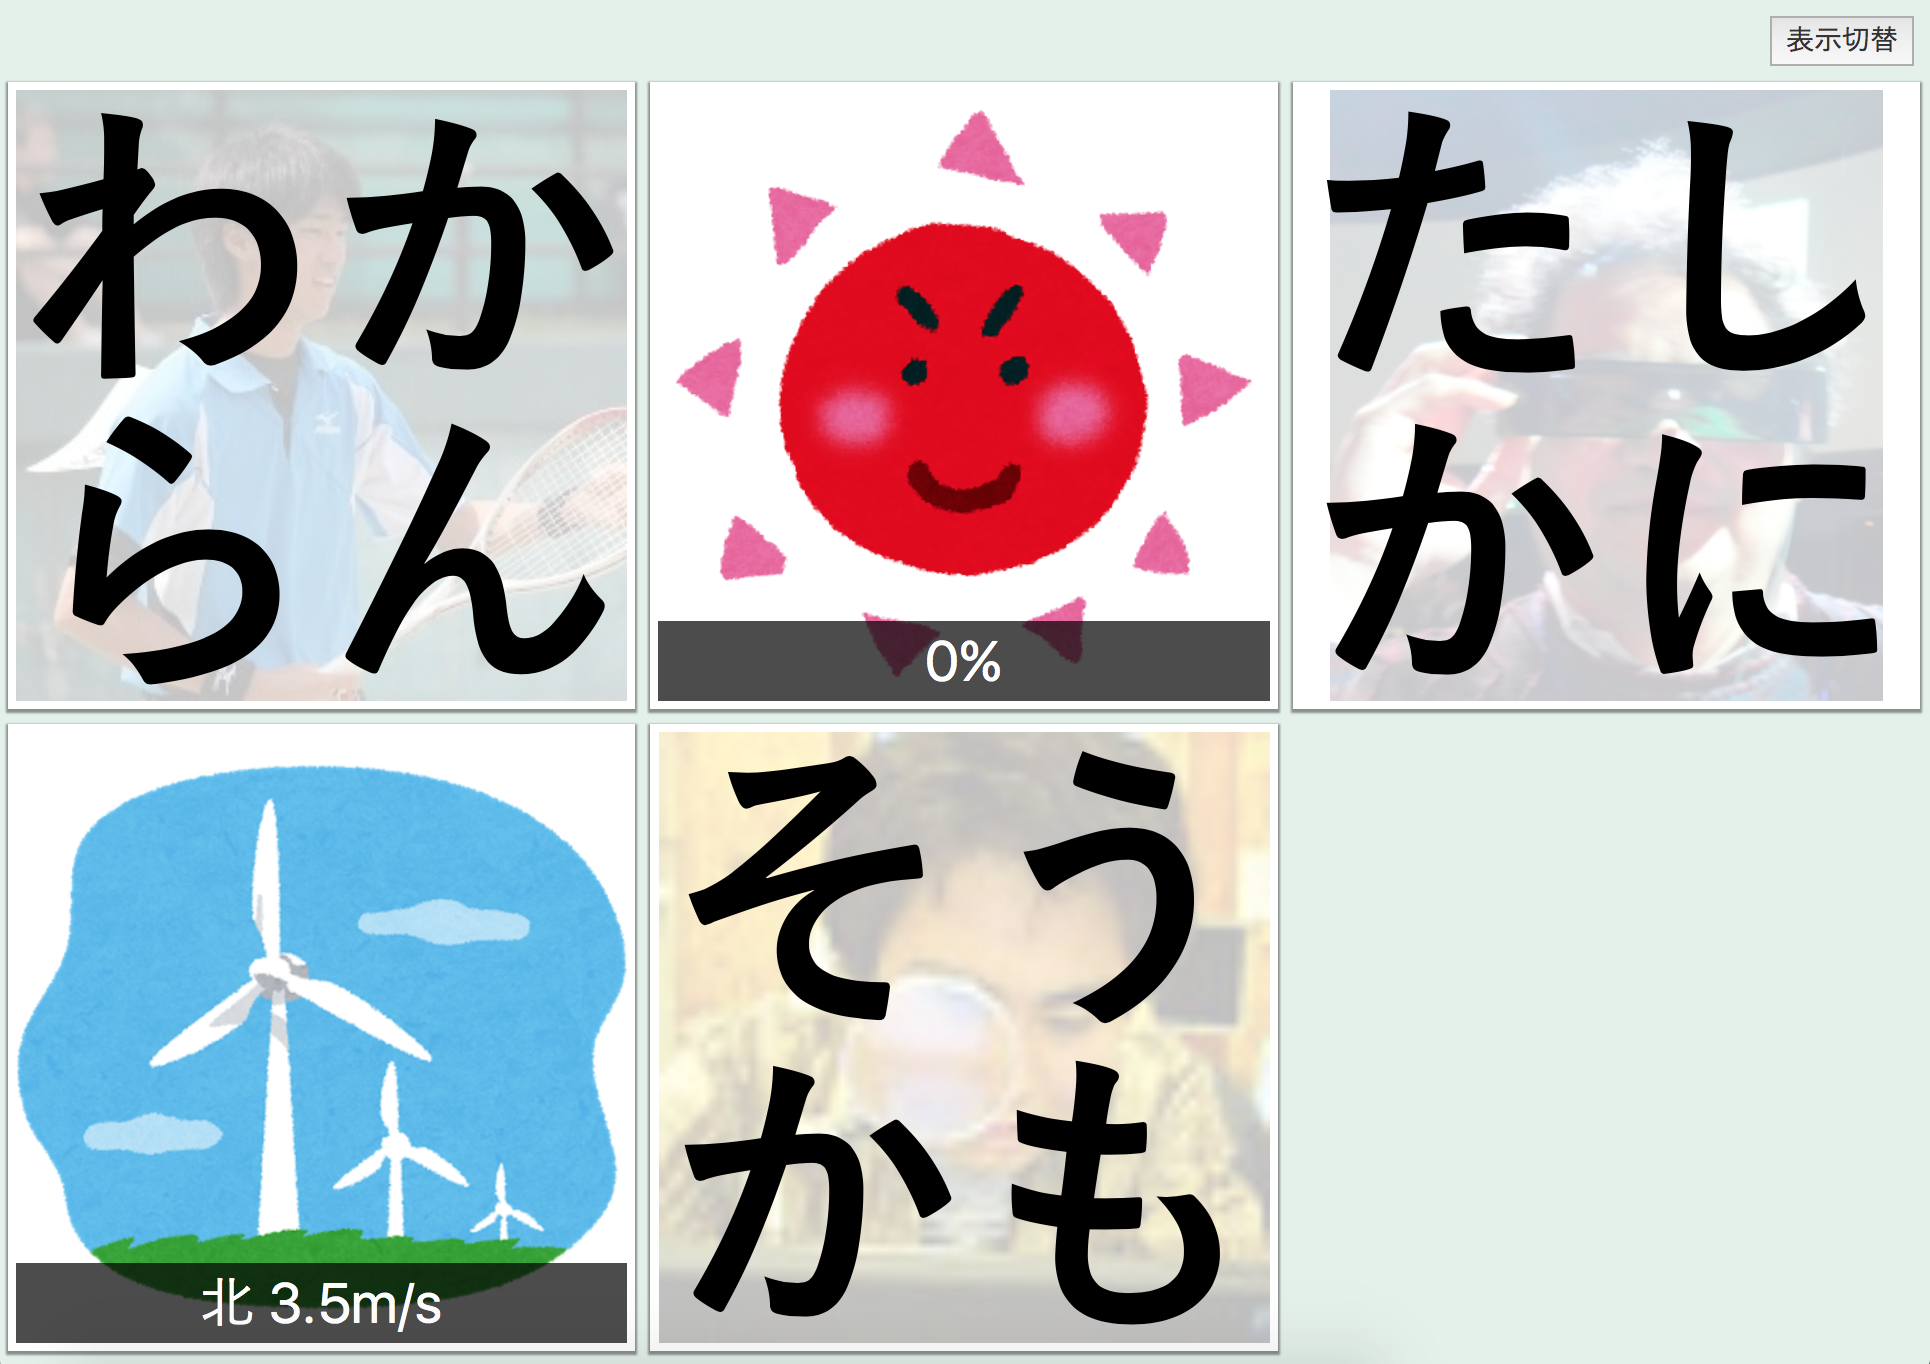
\includegraphics[width=7cm]{images/n_w_m_w_s.png}
\caption{ユーザとデータを表示}
\label{n_w_m_w_s}
\end{figure}

\subsection{スタンプの作成}
ユーザが投稿画面でリアクションとして投稿するスタンプには,
「テキスト」スタンプと「画像」スタンプの2種類がある(図\ref{stamp}).

ユーザは投稿画面のテキストボックスに文字列を入力して追加ボタンを押すことで
スタンプを作成して追加することができる.

画像スタンプは,テキストボックスに\url{http://masuilab.org/image.jpg}のようなWebにある
画像のURLを入力し追加ボタンを押すことで,URLの画像をスタンプとして一覧に追加することができる.
ローカルにある画像ファイルをスタンプとして追加したい場合は,
Gyazo\footnote{https://gyazo.com}などのアプリケーションを使って
WebにアップロードしURLを得ることで追加が可能である.

テキストスタンプは,テキストボックスにURLでないを文字列を入力し追加ボタンを押すことで作成できる.
図\ref{wakaran}左は「わからん」とテキストボックスに入力してスタンプを作成したものである.
この「わからん」は1行に表示されているが,「わか らん」と改行を入れたい場所に空白文字を入力
することで,図\ref{wakaran}右のように2行で表示される.

% スタンプの削除は,スタンプにマウスオーバーすると右上に表示される「×」ボタンを押すことで削除できる.

\begin{figure}[h]
\centering

\includegraphics[width=7cm]{images/stamp.png}
\caption{テキストスタンプ(左)と画像スタンプ(右)}
\label{stamp}
\end{figure}

\begin{figure}[h]
\centering

\includegraphics[width=7cm]{images/wakaran.png}
\caption{「わからん」スタンプ(左)と「わか らん」スタンプ(右)}
\label{wakaran}
\end{figure}

\subsection{利用例}
図\ref{discussion}は会議や発表の場での利用例である.これは誰かが何か変なことを言ったのに対してユーザが反応している様子である.

図\ref{sensors}はダッシュボードとしての利用例で,各種のセンサの値やWebの情報等を表示している.

データはリアルタイムに最新のものに更新されていく.

\begin{figure}[h]
\centering
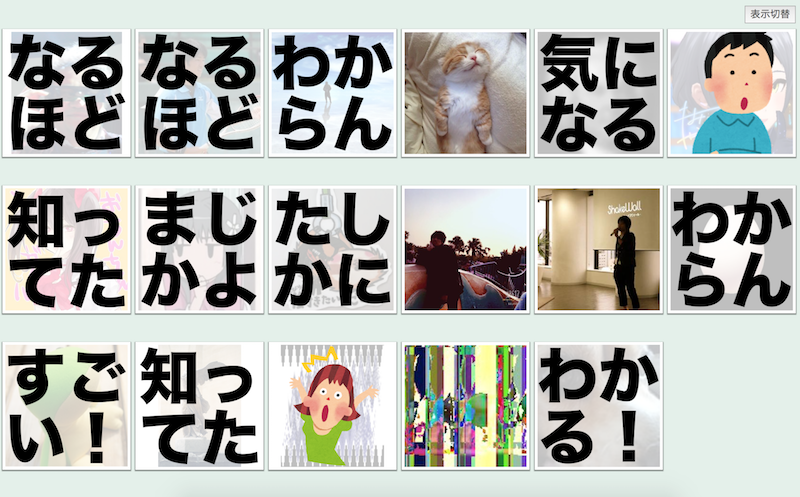
\includegraphics[width=7cm]{images/discussion.png}
\caption{会議や発表の場での利用例}
\label{discussion}
\end{figure}

\begin{figure}[h]
\centering
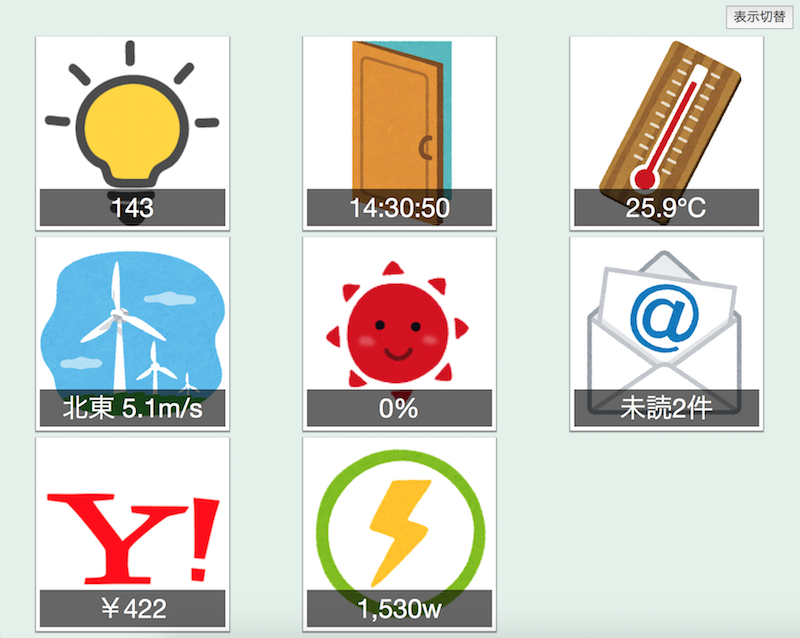
\includegraphics[width=7cm]{images/sensors.png}
\caption{ダッシュボードとしての利用例}
\label{sensors}
\end{figure}
